\maketitle

\
These short notes  (under construction) are meant for the students of the  {\em Optimization} course, with no background in Linear Algebra. Students can check out, for instance, the Linear Algebra textbook of the Schaum series for further examples and exercises. They should, however be familiar with matrix multiplication and  able to solve linear systems.  The  Gauss elimination method is also  described at the beginning of these notes.


\section{Introduction}
Suppose we're trying to build a remote for a DVD player.

% TODO: fill intro

\begin{definition}[Hamming distance]
Given two code words $\textbf{w}, \textbf{w}' \in \{0,1\}^n$, the \emph{Hamming distance} between $\textbf{w}$ and $\textbf{w}'$ is the number of bits in which $\textbf{w}$ differs from $\textbf{w}'$:

\begin{equation}
    d_H(\textbf{w}, \textbf{w}') := |\{j \in \{1, 2, \ldots, n\} : w_j \neq w_j'\}|.
\end{equation}
\end{definition}
In other words, the Hamming distance is the number of errors (bit flips) that need to occur for \textbf{w} to become \textbf{w'}.

\begin{example}
If $n = 3$, we can form $2^3=8$ unique code words, with the following distances from each other:

\begin{table}[!ht]
    \centering
    \begin{tabular}{|c|c|c|c|c|c|c|c|c|}
    \hline
        \textbf{$d_H$} & \textbf{101} & \textbf{111} & \textbf{011} & \textbf{001} & \textbf{000} & \textbf{010} & \textbf{110} & \textbf{100} \\ \hline
        \textbf{101} & 0 & 1 & 2 & 1 & 2 & 3 & 2 & 1 \\ \hline
        \textbf{111} & 1 & 0 & 1 & 2 & 3 & 2 & 1 & 2 \\ \hline
        \textbf{011} & 2 & 1 & 0 & 1 & 2 & 1 & 2 & 3 \\ \hline
        \textbf{001} & 1 & 2 & 1 & 0 & 1 & 2 & 3 & 2 \\ \hline
        \textbf{000} & 2 & 3 & 2 & 1 & 0 & 1 & 2 & 1 \\ \hline
        \textbf{010} & 3 & 2 & 1 & 2 & 1 & 0 & 1 & 2 \\ \hline
        \textbf{110} & 2 & 1 & 2 & 3 & 2 & 1 & 0 & 1 \\ \hline
        \textbf{100} & 1 & 2 & 3 & 2 & 1 & 2 & 1 & 0 \\ \hline
    \end{tabular}
    \caption{Hamming distances for all possible code words with $n=3$}
\end{table}

Another way to visualize the Hamming distance is by putting each possible code word in the vertices of a (hyper)cube. Of course, for $n=2$ the cube becomes a square. If every word is placed such that it has only one bit of difference with respect to each of its neighbors, then the Hamming distance between two words will be the number of edges we need to traverse in order to get from one word to the other.

\begin{figure}
    \centering
    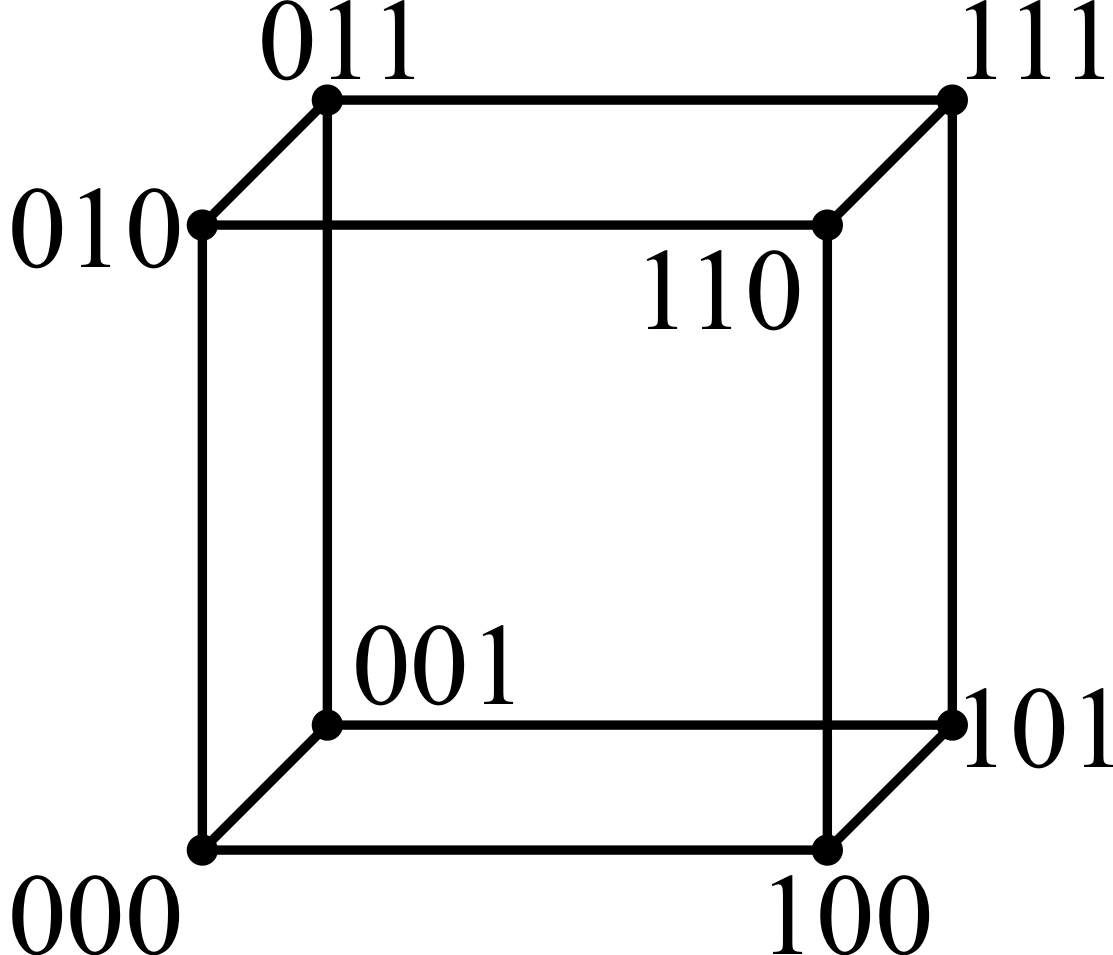
\includegraphics[width=0.25\textwidth]{hamming-cube.png}
\caption{Hamming cube for $n=3$}
\end{figure}

\end{example}

\begin{definition}[weight of a code-word]
Suppose $\textbf{w}$ is a code-word such that $\textbf{w} \in \{0,1\}^n$. The \emph{weight} of $\textbf{w}$ is the number of 1's in $\textbf{w}$:

\begin{equation}
    |\textbf{w}| := |\{j \in \{1, 2, \ldots, n\} : w_j = 1\}|.
\end{equation}

\end{definition}
\begin{example}
Suppose $n=5$.
\begin{equation}
    |(1, 0, 0, 1, 1)| = 3 \quad\quad |(1, 0, 0, 0, 0)| = 1 \quad\quad |(0, 0, 1, 1, 1)| = 4
\end{equation}
\end{example}

\begin{definition}[bit-wise xor]
Given two words $\textbf{w}, \textbf{w}' \in \{0,1\}^n$, we can define the following operation:
\begin{equation}
    \textbf{w} \oplus \textbf{w}' = ((w_1 + w_1')\text{mod}2, (w_2 + w_2')\text{mod}2, \ldots, (w_n + w_n')\text{mod}2) \in \{0,1\}^n
\end{equation}
\end{definition}
The \emph{sum modulo 2} operation returns a vector of size $n$ where each component  $z_j$ has value:
\begin{itemize}
    \item 0 if $w_j = w_j'$;
    \item 1 if $w_j \neq w_j'$
\end{itemize}

\begin{example}
Suppose $n=6, \textbf{w} = (1, 1, 0, 0, 1, 0), \textbf{w}' = (0, 1, 1, 0, 0, 1)$.
\begin{equation}
\begin{array}{l}
(1, 1, 0, 0, 1, 0) \,+ \\
(0, 1, 1, 0, 0, 1) = \\  \hline
(1, 2, 1, 0, 1, 1)
\end{array}
\quad\rightarrow\quad
\begin{array}{l}
(1, 2, 1, 0, 1, 1)\text{mod} 2 = \\ \hline
(1, 0, 1, 0, 1, 1) = \textbf{w} \oplus \textbf{w}'
\end{array}.
\end{equation}
\end{example}

At this point, it's clear how this identity holds true:
\begin{equation}
    d_H(\textbf{w}, \textbf{w}') = |\textbf{w} \oplus \textbf{w}'|
\end{equation}
Which means: the weight of the result obtained from the bit-wise xor operation is the Hamming distance between the two code-words.

\begin{definition}[distance of a code]
In coding theory, any subset $\mathcal{C} \subseteq \{0,1\}^n$ is called a \emph{code}.

A code $\mathcal{C}$ has \emph{distance} $d$ if:

\begin{equation}
    d_H(\textbf{w}, \textbf{w}') \geq d \;\; \forall \;\textbf{w}, \textbf{w}' \in \mathcal{C}.
\end{equation}

Lastly, for $n, d \geq 0$, let $A(n,d)$ denote the maximum cardinality of a code $\mathcal{C} \subseteq \{0,1\}^n$ with distance $d$.
\end{definition}

\begin{example}
For $n=7$, a valid code of distance $d=3$ could be the set:

\begin{equation}
\mathcal{C} =
\left.
\begin{cases}
& 0000000, 0001011, 0010101, 0011110, \;\;\;\\
& 0100110, 0101101, 0110011, 0111000, \\
& 1000111, 1001100, 1010010, 1011001, \\
& 1100001, 1101010, 1110100, 1111111 
\end{cases}\right\}.
\end{equation}

Notice how, in this code, every two distinct words have an Hamming distance of at least $3$.
\end{example}

\begin{proposition}
A code $\mathcal{C}$ can correct at most $r$ errors if and only if it has distance $d \geq 2r+1$.
\end{proposition}
\begin{example}
    Suppose $\mathcal{C}$ contains two distinct words $\textbf{w}', \textbf{w}''$ that differ in at most $2r$ bits. For example, with $n=7$ and $r=1$, suppose we receive $\hat{\textbf{w}}$, obtained by flipping $r=1$ bits in one of them:
\begin{equation}
\textbf{w}' = 0000011 \quad \textbf{w}'' =0000101 \quad \hat{\textbf{w}} = 0000001
\end{equation}
At this point, it's impossible to know whether the originally transmitted word was $\textbf{w}'$ or $\textbf{w}''$. This test can be repeated by choosing any code with distance $d=2r$ and flipping $r$ of them.

On the other hand, if $\mathcal{C}$ had a distance of $2r+1$, we would be sure it could correct up to $r$ errors:

\begin{equation}
\textbf{w}' = 0000011 \quad \textbf{w}'' =0010101 \quad \hat{\textbf{w}} = 0000001
\end{equation}

In this case, we can be sure that $\textbf{w}''$ was transmitted.
\end{example}

In most cases, the number $n$ of bits we can transmit and the amount of errors $r$ to be corrected are given; one of the main problems of coding theory (and the main topic of this document) is finding $A(n,d)$, the maximum possible size of a code $\mathcal{C} \subseteq \{0,1\}^n$ with distance $d$.

\subsection{Simple cases}
For all $n$, we always have $A(n,1) = 2^n$, because any code has distance 1 by definition; of course, this does not allow us to correct any error.
%TODO: finish this part
%\begin{array}{l}

%\end{array};

\subsection{The sphere-packing bound}
For any $n$ and $d$, we can use a \emph{volume argument} to obtain a simple upper bound on $A(n, d)$.

Imagina a spherical box filled with prize balls. If you wanted to guess how many balls can fit inside it, you could conclude that the number of balls is bounded above by the volume of the spherical box divided by the volume of a single box.

Let's assume that $d = 2r+1$ is odd and fix any code $\mathcal{C}$ of distance $d$. Now, the set $\{0,1\}^n$ represents the spherical box, containing $|\mathcal{C}|$ Hamming balls:
\begin{equation}
    B(\mathbf{w}, r) := \{\mathbf{w}' \in \{0,1\}^n : d_H(\mathbf{w}, \mathbf{w}') \leq r\}, \mathbf{w} \in \mathcal{C}.
\end{equation}

\section{The Delsarte Bound}
test
